%!TEX root = ../main.tex

\section{PostgreSQL}
\label{section:postgresql}

PostgreSQL \cite{postgresql} is an open-source object-relational database management [ORDBMS] system based on Postgres, and was developed at the \textit{University of California at  Berkeley Computer Science Department} in 1996.

The name of the system reflects its support for most SQL standards, but the system also offers many advanced features, such as complex queries, foreign keys, triggers, multi-version concurrency control and more. 

PostgreSQL is also highly extensible, which allows users to define new data types, functions, indexing methods and more, without having to modify the core database engines. This feature allows new extensions to be added, capable of handling user-defined data types, while keeping the full power of a traditional database management system [DBMS].

\section{PostGIS}
\label{section:postgis}

PostGIS \cite{postgis}, released in 2001, is one example of an extension to the PostgreSQL DBMS. PostGIS is an open-source spatial extension to PostgreSQL that adds support for a wide range of geographic objects. 

This extension allows \textit{Geographical Information System} [GIS] objects, such as points, linestring or polygons, to be stored in the database. It also includes support for processing and analyzing GIS objects, by defining functions and operations that can be used to process them, such as distance and area functions.

A PostGIS type that will be used a lot in this thesis is the \textit{Polygon} type, since this will be used to represent a static region. A PostGIS polygon object is defined as having an exterior ring, as well as zero or more interior rings, that define holes in the polygon. Figure \ref{fig:polygons} shows some example of polygons that are accepted or rejected by the PostGIS implementation.

\begin{figure}[h!]
    \centering
    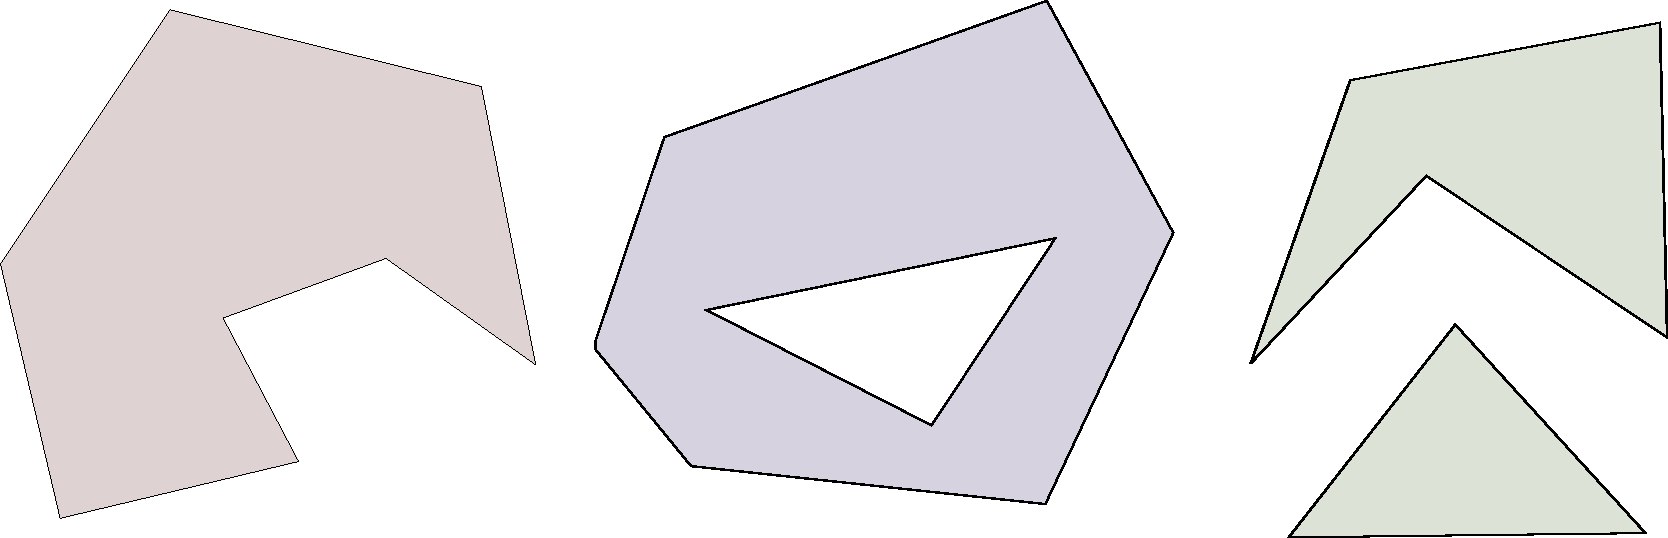
\includegraphics[width=0.75\textwidth]{images/polygons.pdf}
    \caption{Examples of regions that can (brown and purple) or cannot (green) be represented using the PostGIS polygon type.}
    \label{fig:polygons}
\end{figure}

Contrary to most research papers about moving regions \cite{polyhedra,model_structure_for_mod,moving_obj_foundation}, this definition of a region does not allow a region/polygon to have multiple faces, which is usually necessary to be able to describe regions that split or merge together. PostGIS allows the creation of multi-polygons, which could theoretically be used to describe a region made of multiple faces, but since in our case we will only handle non-deforming (fixed-shape) regions, there will be no need for polygons to merge or split, so this will not be discussed further.

\section{MobilityDB}
\label{section:mobilitydb}

MobilityDB \cite{mobilitydb} is an extension to PostgreSQL and PostGIS that provides \textit{temporal types}, used to represent the evolution on time of some base type. For example, the temperature of a room can be represented by a real value that changes through time. In this case, the temporal type is a \textit{temporal float}, with the base type being \textit{float}. As another example, a \textit{temporal integer} can be used to represent the number of people on a train. Similarly, a \textit{temporal point} can be used to store the position of a taxicab, as reported by a GPS device.

MobilityDB makes use of the predefined operations on the base type, such as arithmetic operations and aggregations for integers and floats or spatial functions for geometries, to define new operations that can handle temporal types.

MobilityDB uses four time types to represent extents of time: \textit{timestamptz}, \textit{timestampset}, \textit{period} and \textit{periodset}. Timestamptz is a PostgreSQL type, while the three other types are new. Two new range types are also defined in MobilityDB: \textit{intrange} and \textit{floatrange}

\subsection{Temporal Types}
\label{section:mobilitydb_ttypes}

There are six existing temporal types, \textit{tbool}, \textit{ttext}, \textit{tint}, \textit{tfloat}, \textit{tgeompoint} and \textit{tgeogpoint}, based on, respectively, the base types bool, text, int, float, geometry(Point) and geography(Point). The last two are the PostGIS types for points, restricted to 2D and 3D.

Temporal types can have four possible duration: Instant, Instant Set, Sequence and Sequence Set. These durations define the temporal extent at which the evolution of values is defined.

\subsubsection{Temporal Instant}
\label{section:mobilitydb_inst}

A temporal instant represents the value of an object at a particular timestamp using the following notation:

\[
    'v@t'
\]

, where \(v\) is the value and \(t\) is the timestamp.

For example, if we want to store the fact that the temperature of a room was 21 (degrees Celsius) on September 1st 2019 at midnight, we will store this as:

\[
    '21@\text{2019-01-01 00:00:00}'
\]

\subsubsection{Temporal Instant Set}
\label{section:mobilitydb_i}

As the name hints, temporal instant sets are simply sets of temporal instants. Temporal objects of instant set duration are used to represent a value that is defined at multiple instants in time, without being defined in between these instants. For example, a temporal instant set composed of 3 instants will be written as:

\[
    '\{v_0@t_0,\ v_1@t_1,\ v_2@t_2\}'
\]

, where \(v_i\) are the values and \(t_i\) are the timestamps in increasing order \(t_i < t_{i+1}\).

The value of this object is thus defined only at the given timestamps, and no assumptions are made for intermediate timestamps.

\subsubsection{Temporal Sequence}
\label{section:mobilitydb_seq}

A temporal sequence is defined just as a a temporal instant set, except that the values for intermediate timestamps can be obtained by interpolation. The value of the temporal object is thus assumed to be defined over the whole period of the sequence.

Depending on the base type of the object, two interpolation methods are possible, stepwise/discrete or linear/continuous. The base types bool, text, and integer are forced to use a discrete interpolation method, whereas the base types float, geometry and geography can use either one depending on the use case.

For example, when using a \textit{tint} to represent the number of people in a bus, if a new temporal instant is added every time someone steps in or out of the bus, we can get the number of people in the bus at any time during its trip, by simply looking at the latest defined value before that instant. This is an example of a stepwise interpolation for temporal integers.

An example of a linear interpolation could be the case of a room thermometer. If we measure the temperature sufficiently often, we can assume that the temperature between two measures can be obtained by interpolating linearly between these two values. These measurements will thus be stored in a temporal sequence with float base type, and intermediate values will be retrieved using a linear interpolation method.

A temporal sequence composed of 3 instants is written as:

\[
    '[v_0@t_0,\ v_1@t_1,\ v_2@t_2]'
\]

, with again \(t_i < t_{i+1}\).

A temporal sequence has a lower and upper bound that can be either inclusive (represented by '[' and ']') or exclusive (represented by '(' and ')').

\subsubsection{Temporal Sequence Set}
\label{section:mobilitydb_s}

A temporal value of sequence set duration represents the evolution of the value over a set of sequences, with the value between these sequences being unknown. A temporal sequence set with 2 sequences of 2 instants each will be written as:

\[
    '\{[v_0@t_0,\ v_1@t_1],\ [v_2@t_2,\ v_3@t_3]\}'
\]

, where the same inclusion/exclusion rules as for sequences apply.

It would theoretically be enough to only implement the temporal sequence set type, since all three previous types are essentially special cases of this one, but for efficiency reasons all four types exist.

\subsection{Bounding Box}
\label{section:mobilitydb_bbox}

Each temporal object also has an associated bounding box, whose type depends on the base type of the object. The following bounding box types exist:

\begin{itemize}
    \item Period: for the types \textit{tbool} and \textit{ttext}, where only the temporal extent is taken into account.
    \item Tbox (temporal box): for the types \textit{tint} and \textit{tfloat}, where the value extent is stored in the X dimension, and the temporal extent in the T dimension.
    \item STbox (spatio-temporal box): for the types \textit{tgeompoint} and \textit{tgeogpoint}, where the spatial extent stored in the X, Y and Z dimension, and the temporal extent in the T dimension.
\end{itemize}

These bounding boxed are used instead of the temporal object itself in some operations, in particular those related to indexing, for efficiency reasons.

\subsection{Functions and Operators for Temporal Types}
\label{section:mobilitydb_functions}

MobilityDB exposes a large set of functions and operators for temporal types. These functions and operators are polymorphic, meaning they can have arguments of several types and the result type may vary depending on the input types, and they can be grouped into the categories described below. 

Note that this list is only there to introduce the set of functions exposed by MobilityDB, and does not consist of an exhaustive list of all available functions. For a more complete and detailed list, refer to the MobilityDB manual \cite{mobiliydb_manual}.

\begin{itemize}
    \item Transformation Functions:

        These functions are used to transform a temporal value into another duration. If the transformation is not possible, an error will be raised. 

        Ex.: tintseq:
        \begin{flalign*}
            & \text{SELECT tintseq(tint }'1@\text{2001-01-01}'\text{);}     &&\\
            & \text{- - }"[1@\text{2001-01-01}]"                            &&
        \end{flalign*}

        Appending a temporal instant to the temporal value, and merging two temporal values of the same duration, is also a part of the transformation functions.

        Ex.: appendInstant:
        \begin{flalign*}
            & \text{SELECT appendInstant(tint }'1@\text{2001-01-01}',\ \text{tint }'1@\text{2001-01-02}'\text{);}     &&\\
            & \text{- - }"\{1@\text{2001-01-01},\ 1@\text{2001-01-02}\}"                            &&
        \end{flalign*}

    \item Accessor Functions:

        A multitude of accessor functions exist, that enable the retrieval of a particular instant, timestamp or value from the temporal value. The duration or memory size of the value can also be retrieved.

        Some example functions are shown below:

        Ex. 1: memsize:
        \begin{flalign*}
            & \text{SELECT memsize(tint }'[1@\text{2001-01-01},\ 2@\text{2001-01-02},\ 1@\text{2001-01-03}]'\text{);}     &&\\
            & \text{- - }280                            &&
        \end{flalign*}

        Ex. 2: getValue:
        \begin{flalign*}
            & \text{SELECT duration(tint }'1@\text{2001-01-01}'\text{);}     &&\\
            & \text{- - }1                            &&
        \end{flalign*}

        Ex. 3: instantN:
        \begin{flalign*}
            & \text{SELECT instantN(tint }'[1@\text{2001-01-01},\ 2@\text{2001-01-02},\ 1@\text{2001-01-03}]', \ 2\text{);}     &&\\
            & \text{- - }"2@\text{2001-01-02}"                            &&
        \end{flalign*}

    \item Spatial Functions

        Spatial functions that can be applied to temporal points. Most of the functions support 3D points, and/or are available for geographies.

        These functions range from output in specific format (ex: \textit{EWK} or \textit{MFJSON}), to more complicated accessor functions, such as \textit{speed} or \textit{nearestApproachDistance}.

        Ex.: speed:
        \begin{flalign*}
            & \text{SELECT speed(tgeompoint }'[\text{Point}(1\ 0)@\text{2001-01-01},\ &&\\
            & \eqtab\text{Point}(1\ 0)@\text{2001-01-02},\ \text{Point}(1\ 1)@\text{2001-01-03}]') * 3600 * 24;     &&\\
            & \text{- - }"\{[0@\text{2001-01-01}, 0@\text{2001-01-02}),\ [1@\text{2001-01-02}, 1@\text{2001-01-03}]\}"                            &&
        \end{flalign*}

    \item Restriction Functions:

        These functions restrict a temporal value, either on its value extent or its time extent.
        Example of restriction functions are: \textit{atValue}, \textit{atMax}, \textit{atPeriod}, etc.

        Ex.: atMax:
        \begin{flalign*}
            & \text{SELECT atMax(tint }'[1@\text{2001-01-01},\ 2@\text{2001-01-02},\ 1@\text{2001-01-03}]'\text{);}     &&\\
            & \text{- - }"\{[2@\text{2001-01-02}]\}"                            &&
        \end{flalign*}

    \item Difference Functions:

        These functions act similarly to the restriction functions, except that they restrict the temporal value to the complement of a value or a time extent.

        Ex.: minusValue:
        \begin{flalign*}
            & \text{SELECT minusValue(tint }'[1@\text{2001-01-01},\ 2@\text{2001-01-02},\ 1@\text{2001-01-03}]',\ 2);     &&\\
            & \text{- - }"\{[1@\text{2001-01-01},\ 1@\text{2001-01-02}),\ [1@\text{2001-01-03}]\}"                            &&
        \end{flalign*}

    \item Comparison Operators

        Implementation of the traditional comparison operators ('$=$', '$<$' and so on). Except for equality and inequality, these are not useful for real-world use cases, but they allow the construction of B-tree indexes on temporal types. 

    \item Ever and Always Equals Operators

        These operators test whether a temporal value is ever equal ('$\&=$') or always equal ('$@=$') to a value.

    \item Temporal Comparison Operators

        These comparison operators are generalization of the traditional comparison operators, and return a \textit{tbool} value.

        Ex.: temporal not equal, $\#<>$:
        \begin{flalign*}
            & \text{SELECT tint }'[1@\text{2001-01-01},\ 4@\text{2001-01-04}]'\ \#<> 2;     &&\\
            & \text{- - }"\{[t@\text{2001-01-01},\ f@\text{2001-01-02},\ t@\text{2001-01-03},\ t@\text{2001-01-04}]\}"                            &&
        \end{flalign*}

    \item Mathematical Function Operators

        The basic mathematical functions, such as addition, multiplication, rounding and more.

    \item Boolean Operators

        Boolean \textit{and}, \textit{or} and \textit{not}.

    \item Text Functions and Operators

        Text concatenation, lowercase and uppercase.

    \item Bounding Box Operators

        These are the comparison operators on the corresponding bounding boxes of temporal values. Operators exist for different kind of relationships (for example: less than, contains, overlaps, equal, etc) and for all possible dimensions of the bounding boxes (value/X, Y, Z and T dimension). As said previously, the Y and Z dimensions are only used in case of temporal points. These functions all return a boolean value.

        Ex.: Bounding box overlap, $\&\&$:
        \begin{flalign*}
            & \text{SELECT tint }'[1@\text{2001-01-01},\ 4@\text{2001-01-04}]'\ \&\&\ 2;     &&\\
            & \text{- - true}                            &&
        \end{flalign*}

    \item Distance Operators

        Computes the distance between two temporal points as a tfloat ('\(<->\)') or the smallest distance between two temporal points as a float ('\(|=|\)'). Since the distance function quadratic, the distance operator uses a linear approximation of the usual distance functions, to be able to return a tfloat.

    \item Spatial Relationships for Temporal Points

        The PostGIS spatial relationships functions (such as \textit{ST\_Intersects} and \textit{ST\_Relate}) are generalized in two different ways. In the first version the PostGIS functions are applied to the union of all values taken by a temporal point (ex. \textit{intersects} and \textit{relate}). The second version is defined with temporal semantics and returns a temporal value. For the two example functions, the second version is \textit{tintersects} and \textit{trelate}, which return a \textit{tbool} and a \textit{ttext} respectively.

    \item Aggregate Functions for Temporal Types

        These are the generalization of the usual aggregation functions, such as \textit{tcount}, \textit{tmax}, etc. The generalized form is defined with temporal semantics, and return a temporal value.

\end{itemize}

\subsection{Additional Notations}
\label{section:mobilitydb_notations}

When talking specifically about a temporal type of instant duration, we will add a suffix \textit{inst} to the name of the type. For example a temporal float of instant duration will be denoted \textit{tfloatinst}. 
Similarly, for temporal instants of instant set, sequence and sequence set duration, we will add respectively the suffix \textit{i}, \textit{seq} and \textit{s}. For the base type float, this will thus become: \textit{tfloati}, \textit{tfloatseq} and \textit{tfloats}.